\documentclass[aspectratio=169 %可调屏宽比16:9(169),4:3(43)
,serif,mathserif]{beamer}

\mode<presentation>{
%\usetheme{default}
%\usetheme{AnnArbor}
%\usetheme{Antibes}
%\usetheme{Bergen}
%\usetheme{Berkeley}
%\usetheme{Berlin}
%\usetheme{Boadilla}
%\usetheme{CambridgeUS}
%\usetheme{Copenhagen}
%\usetheme{Darmstadt}
%\usetheme{Dresden}
%\usetheme{Frankfurt}
%\usetheme{Goettingen}
%\usetheme{Hannover}
%\usetheme{Ilmenau}
%\usetheme{JuanLesPins}
%\usetheme{Luebeck}
\usetheme{Madrid}
%\usetheme{Malmoe}
%\usetheme{Marburg}
%\usetheme{Montpellier}
%\usetheme{PaloAlto}
%\usetheme{Pittsburgh}
%\usetheme{Rochester}
%\usetheme{Singapore}
%\usetheme{Szeged}
%\usetheme{Warsaw}
% As well as themes, the Beamer class has a number of color themes
% for any slide theme. Uncomment each of these in turn to see how it
% changes the colors of your current slide theme.
%\usecolortheme{albatross}
%\usecolortheme{beaver}
%\usecolortheme{beetle}
%\usecolortheme{crane}
%\usecolortheme{dolphin}
%\usecolortheme{dove}
%\usecolortheme{fly}
%\usecolortheme{lily}
%\usecolortheme{orchid}
%\usecolortheme{rose}
%\usecolortheme{seagull}
%\usecolortheme{seahorse}
%\usecolortheme{whale}
%\usecolortheme{wolverine}
%\setbeamertemplate{footline} % To remove the footer line in all slides uncomment this line
%\setbeamertemplate{footline}[page number] % To replace the footer line in all slides with a simple slide count uncomment this line
%\setbeamertemplate{navigation symbols}{} % To remove the navigation symbols from the bottom of all slides uncomment this line
}
\usepackage{adjustbox}
\usepackage{indentfirst} 
\usepackage{amsmath, amsfonts, epsfig, xspace}
\usepackage{algorithm,algorithmic}
\usepackage{beamerthemesplit}
\usepackage{booktabs}
\usepackage{bm}
\usepackage{braket}
\usepackage{calligra}
\usepackage{color}
\usepackage[T1]{fontenc}
\usepackage{fontspec}
\usepackage{ctex}
\usepackage{latexsym}
\usepackage{multicol}
\usepackage{multimedia}
\usepackage{calligra} \DeclareMathAlphabet{\mathcalligra}{T1}{calligra}{m}{n} \DeclareFontShape{T1}{calligra}{m}{n}{<->s*[2.2]callig15}{}
\usepackage{pstricks,pst-node}
\usepackage{ragged2e}
\usepackage{setspace}
\usepackage[normal,tight,center]{subfigure}
\setlength{\subfigcapskip}{-.5em}
\setlength{\parindent}{2em}
\begin{document}
\title{Incremental Maximum Satisfiability} % The short title appears at the bottom of every slide, the full title is only on the title page
\author[Chi~Zhiming]{Reporter:~Chi~Zhiming} % Your name
\institute[ISCAS] % Your institution as it will appear on the bottom of every slide, may be shorthand to save space
{	
	%Lanzhou University \\ % Your institution for the title page
	%\medskip
	%\textit{chizhm16@lzu.edu.cn} % Your email address
}
	\CTEXoptions[today=old]
	\date{\today} % Date, can be changed to a custom date
\begin{frame}[plain]\vspace{1.5em}
\titlepage\vspace{-0.5cm}
%\centerline{\includegraphics[height=0.30\textheight]{logo.png}}
%\hfill 指导教师:xxx
\end{frame}
\begin{frame}{目录}
\tableofcontents
\end{frame}
\AtBeginSection[]
{
\begin{frame}{\tiny}
\frametitle{目录}
\tableofcontents[currentsection]
\end{frame}
}
%----------------------------------------------------------------------------------------
%	PRESENTATION SLIDES
%----------------------------------------------------------------------------------------

%------------------------------------------------
\section{Introduction} % Sections can be created in order to organize your presentation into discrete blocks, all sections and subsections are automatically printed in the table of contents as an overview of the talk
%------------------------------------------------

\setbeamercovered{transparent} 
\begin{frame}{Contribution}
\begin{enumerate}
	\item Detail \textbf{various forms of incrementality in MaxSAT } 
	\begin{itemize}
		\item adding hard clauses, soft literals, assumptions
	\end{itemize} \pause
	\item Propose \textbf{IPAMIR: incremental API for MaxSAT}
	\begin{itemize}
		\item generic interface for developing incremental MaxSAT solvers and applications making use of incremental MaxSAT
		\item MaxSAT Evaluation 2022: incremental track
	\end{itemize} \pause
	\item Develop a fully-fledged \textbf{incremental MaxSAT solver}
	\begin{itemize}
		\item support for all functionality specified in IPAMIR
		\item extends MaxHS: the state-of-the-art implicit hitting set based solver
	\end{itemize} \pause
	\item Provide \textbf{empirical evidence on benefits of incrementality}
	\begin{itemize}
		\item solving under different sets of assumptions
	\end{itemize} 	
\end{enumerate}
\end{frame}

\begin{frame}
	\frametitle{Incremental Optimization}
	\begin{itemize}
		\item Various problem domains call for iterative solving procedures where \textbf{a sequence of related instances are solved}
		\begin{itemize}
			\item adding or removing constraints
			\item modifying objective function
		\end{itemize} \pause
		\item Solving each instance from scratch often too costly: \textbf{reuse information obtained during previous calls} \pause
		\item Incremental SAT solving well-established
		\begin{itemize}
			\item extensively applied by MaxSAT solvers, QBF solvers, etc.
		\end{itemize} \pause
		\item Currently \textbf{MaxSAT solvers offer limited support} for incrementality
		% \begin{itemize}
		% 	\item despite potentially useful information that could be preserved across solver invocations: state of SAT solver, cores
		% \end{itemize}
	\end{itemize}
\end{frame}

\begin{frame}
	\frametitle{MaxSAT}
	\begin{itemize}
		\item Optimization extension of SAT
		\item An instance consists of
		\begin{itemize}
			\item a set of hard clauses $\mathcal{F}_H$,
			\item a set of soft literals $S$,
			\item a weight function $w$ over soft literals $S$.
		\end{itemize}
		\item Find $\tau$ that satisfies all hard clauses and minimizes $\sum_{b \in S} w(b) \cdot b$. \pause
		\item Definition equivalent to weighted soft clauses $\mathcal{F}_L$:
		\begin{itemize}
			\item relax each soft clause $C \in \mathcal{F}_L$ to $C \vee  b_C$.
			\item add $C \vee b_C$ to $\mathcal{F}_H$, and $\neg b_C$ to $S$ with weight $w\left(b_C\right)=w(C)$.
		\end{itemize}
		\item Assumptions $A$: A set of literals
		\item MaxSAT instance $\mathcal{F}$ under a set of assumptions:
			\begin{itemize}
				\item $\mathcal{F} \wedge A=\left(\mathcal{F}_H \wedge \bigwedge_{l \in A}(l), \mathcal{F}_L, w\right)$
			\end{itemize}
	\end{itemize}
\end{frame}

\begin{frame}
	\frametitle{Example 1}
	\begin{figure}[htbp]
		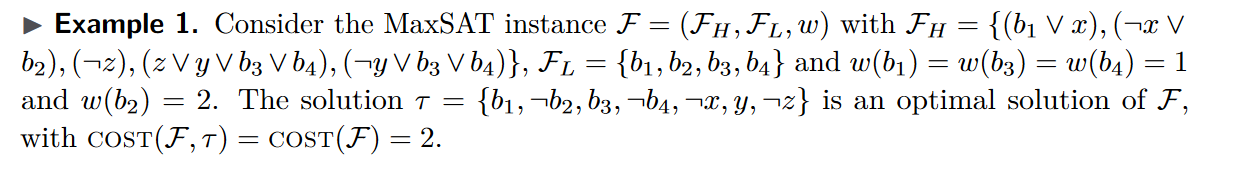
\includegraphics[width=1\linewidth]{1.png}
	\end{figure}
\end{frame}

\begin{frame}
	\frametitle{Incremental changes in MaxSAT}
	\begin{itemize}
		\item Aim for solving a sequence of related MaxSAT instances efficiently, avoiding computation from scratch
		\item Different forms of incremental changes:		
	\end{itemize}
	\begin{figure}[htbp]
		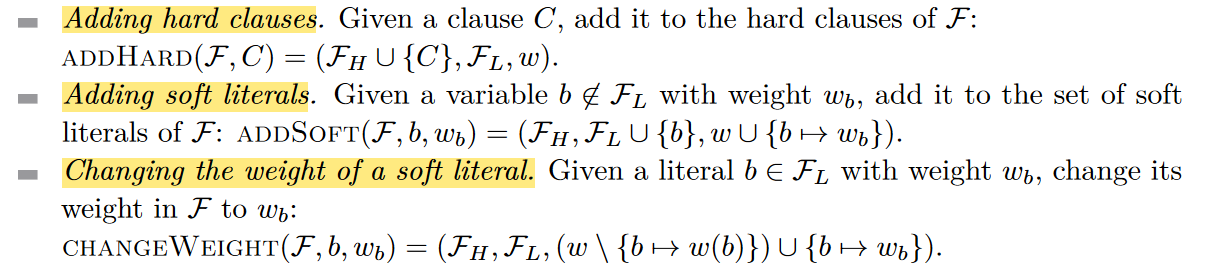
\includegraphics[width=1\linewidth]{2.png}
	\end{figure}
\end{frame}

\begin{frame}
	\frametitle{Incremental changes in MaxSAT}
	\begin{itemize}
		\item Different scenarios call for different forms of incremental changes
		\begin{itemize}
			\item adding hard clauses: MaxSAT-based CEGAR \\
			\qquad\textcolor{blue}{Mangal, Zhang, Nori, and Naik [2015]; Niskanen and Järvisalo [2020]}
			\item changing weights of soft literals: AdaBoost \\
			\qquad\textcolor{blue}{Hu, Siala, Hebrard, and Huguet [2020]}
			\item solving under assumptions: timetabling with disruptions \\
			\qquad\textcolor{blue}{Lemos, Monteiro, and Lynce [2020]}
		\end{itemize}
		\item Assumptions can be used to simulate the removal of clauses and hardening soft clauses.	
	\end{itemize}
\end{frame}

\begin{frame}
	\frametitle{Example 2}
	\begin{figure}[htbp]
		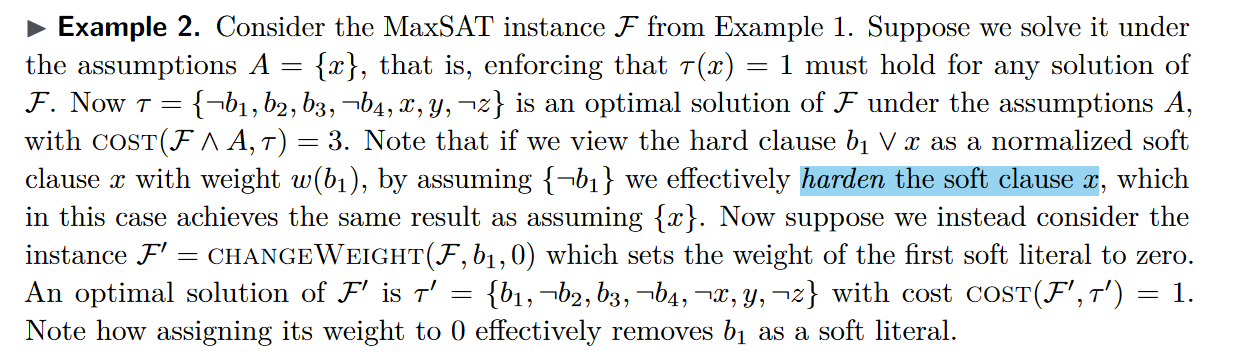
\includegraphics[width=1\linewidth]{3.png}
	\end{figure}
\end{frame}

\section{IPAMIR: Interface for Incremental MaxSAT Solving}
\begin{frame}
	\frametitle{IPAMIR: Interface for Incremental MaxSAT Solving}
	\begin{itemize}
		\item \textbf{Generic interface} for incremental MaxSAT
		\begin{itemize}
			\item for MaxSAT solvers providing support for incrementality
			\item for applications making use of incrementality
		\end{itemize} \pause
		\item Builds on \textbf{IPASIR}: standard interface for incremental SAT \pause
		\item Specifies \textbf{incremental changes} to a MaxSAT instance 
		\begin{itemize}
			\item adding hard clauses
			\item adding soft literals or changing their weights
			\item assumptions on variables
		\end{itemize} \pause		
		\item Includes other essential declarations
		\begin{itemize}
			\item constructing and releasing a solver
			\item solving, variable assignments, objective values
		\end{itemize}
	\end{itemize}
\end{frame}

\begin{frame}
	\begin{figure}[htbp]
		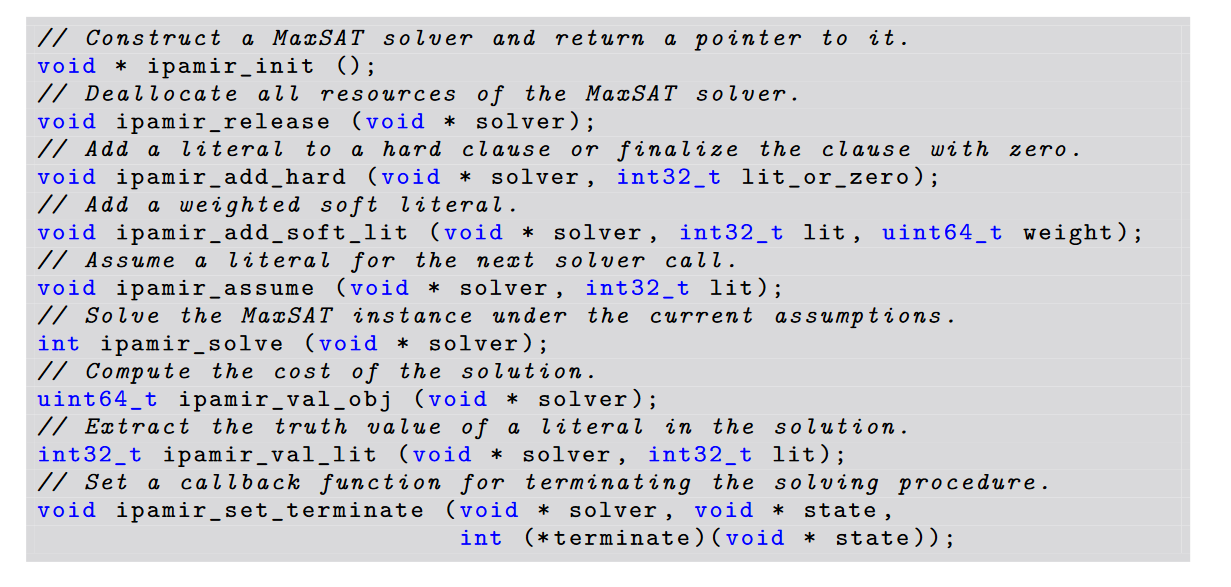
\includegraphics[width=0.9\linewidth]{4.png}
	\end{figure}
\end{frame}

\begin{frame}
	\frametitle{IPAMIR: Interface for Incremental MaxSAT Solving}
	\begin{figure}[htbp]
		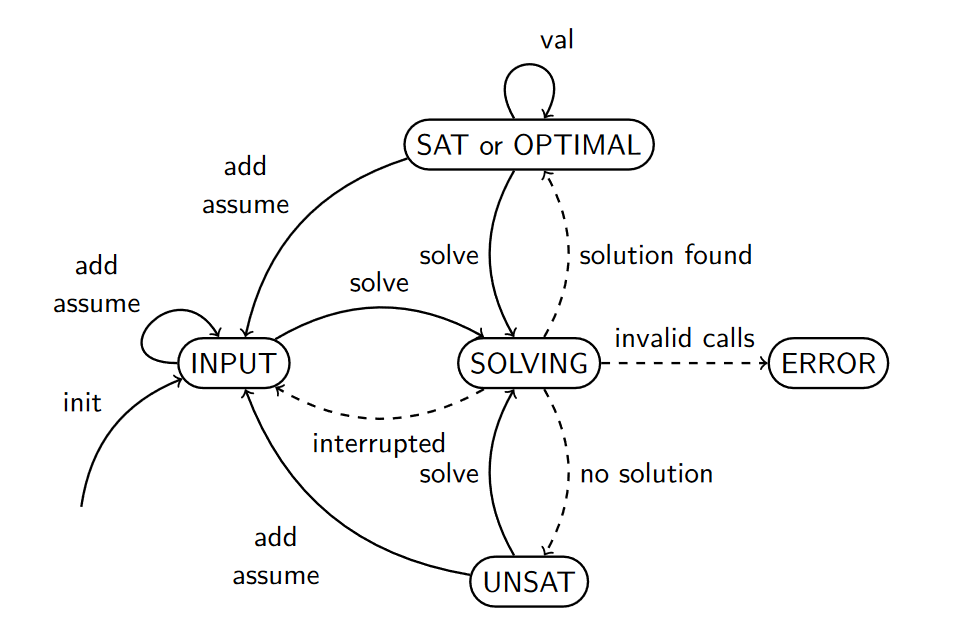
\includegraphics[width=0.6\linewidth]{5.png}
	\end{figure}
\end{frame}

\section{Implicit Hitting Set (IHS) based MaxSAT solving}
\begin{frame}
	\frametitle{Implicit Hitting Set (IHS) based MaxSAT solving}
	\begin{itemize}
		\item An iterative approach: identify \textcolor{blue}{sources of inconsistency} and repair the inconsistencies in a minimal way.
		\begin{itemize}
			\item A \textcolor{blue}{(unsat)core} is a clause over soft literals entailed by the hard clauses.
			\begin{itemize}
				\item SAT solver as core extractor
			\end{itemize} \pause
			\item hs is a hitting set over a set of cores $\mathcal{C}$ if $hs$ intersects each $\kappa \in \mathcal{C}$
			\begin{itemize}
				\item cost of a hitting set determined by weights of soft literals
				\item IP solver for computing minimum-cost hitting sets
			\end{itemize} 
		\end{itemize} \pause
		\item Reasoning and optimization effectively decoupled:
		\begin{itemize}		
			\item upper bounds from assignments given by the SAT solver
			\item lower bounds from costs of optimal hitting sets
		\end{itemize}
	\end{itemize}
\end{frame}

\begin{frame}
	\frametitle{Implicit Hitting Set (IHS) based MaxSAT solving}
	\begin{figure}[htbp]
		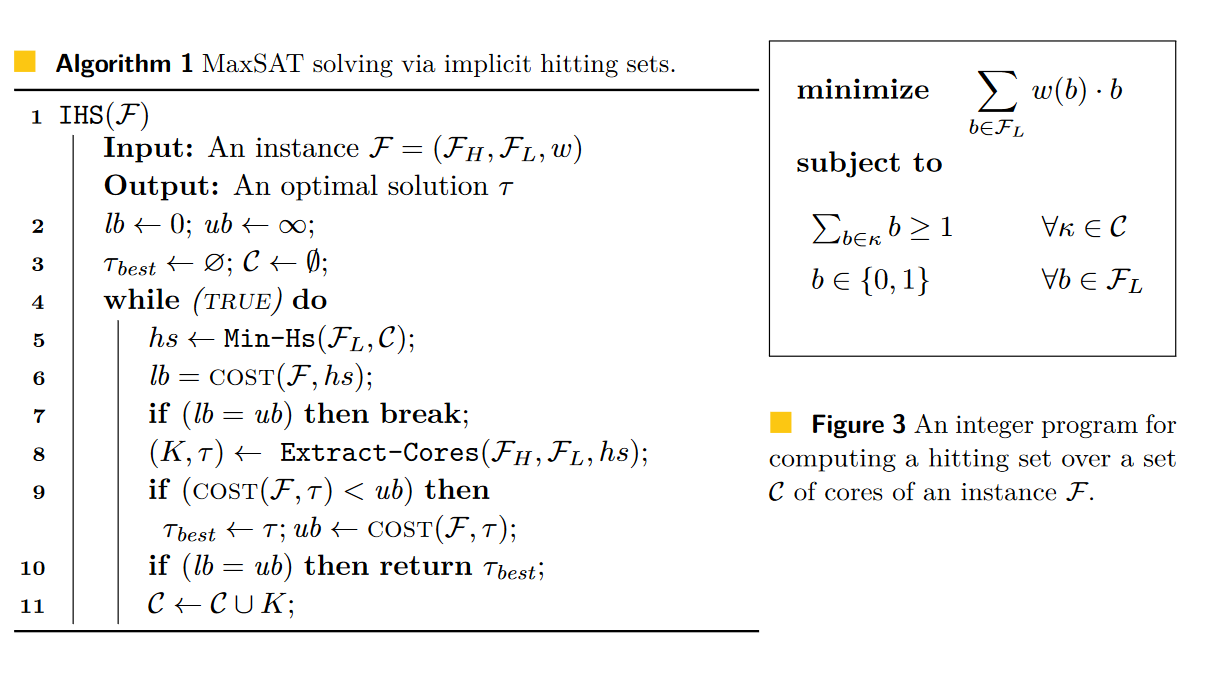
\includegraphics[width=0.7\linewidth]{6.png}
	\end{figure}
\end{frame}

\begin{frame}
	\frametitle{Example 1}
	\begin{figure}[htbp]
		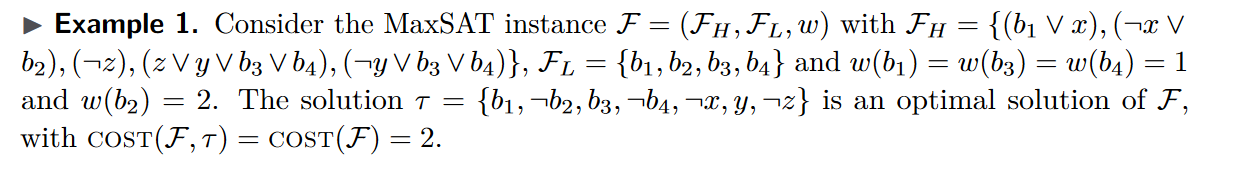
\includegraphics[width=1\linewidth]{1.png}
	\end{figure}
\end{frame}

\begin{frame}
	\frametitle{Example 3}
	\begin{figure}[htbp]
		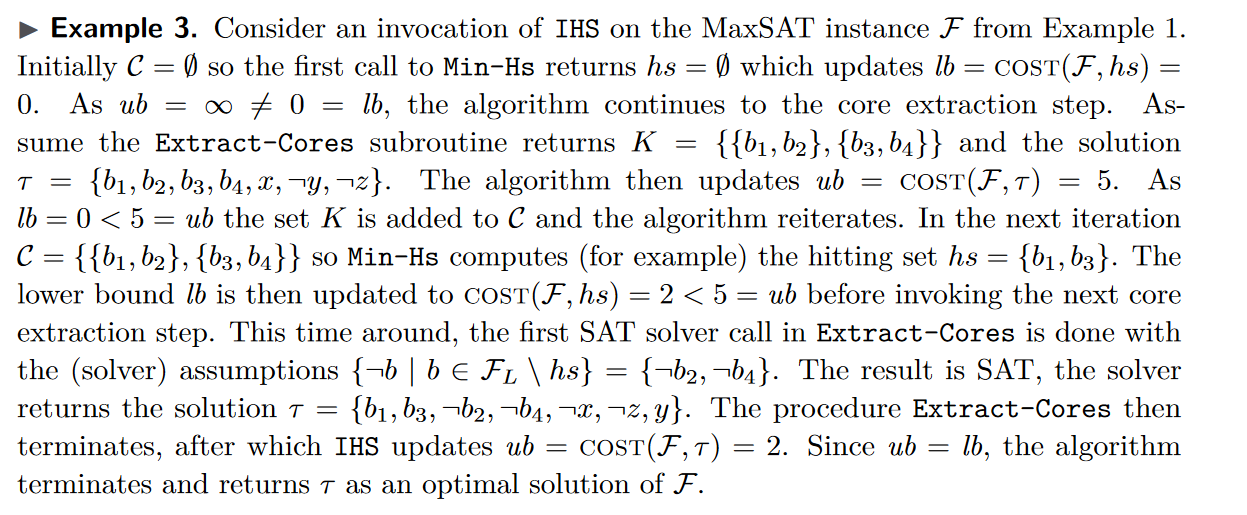
\includegraphics[width=0.8\linewidth]{7.png}
	\end{figure}
\end{frame}

\section{Incremental IHS}
\begin{frame}
	\frametitle{In theory}
	Observations:
	\begin{itemize}
		\item If we add a new hard clause, a new soft literal, or change the weight of a soft literal, all extracted cores are still valid
		\begin{itemize}
			\item cores can be preserved between solver invocations
			\item only objective needs to be altered in the IP solver
		\end{itemize}
		\item The SAT solver knows nothing about the weights of soft literals
		\begin{itemize}
			\item add hard clauses directly to the SAT solver
			\item no need to reinitialize
		\end{itemize}
	\end{itemize} \pause
	How to deal with assumptions without restarting the SAT solver?
\end{frame}



\begin{frame}
	\frametitle{In theory}
	Main idea: pass user-provided assumptions $A$ along with IHS solving assumptions $\neg(\mathcal{F}_L \backslash h s)$ to the internal SAT solver
	\begin{itemize}
		\item if $a \in A \cap \mathcal{F}_L$, do not include $\neg a$ as assumption from $\neg(\mathcal{F}_L \backslash h s)$
		\item cores extracted during search may also contain literals from $\neg A$
		\begin{itemize}
			\item How to preserve cores when solving under assumptions?
		\end{itemize}
	\end{itemize} \pause
	\begin{block}{Conditional Cores}
		Given a MaxSAT instance $\left(\mathcal{F}_H, S, w\right)$, a conditional core with respect to assumptions $A$ is a clause $\kappa^a \subset \neg A \cup S$ that is entailed by $F_H$.
The restriction of a conditional core is $\kappa^a \backslash \neg A$.
	\end{block}
\end{frame}

\begin{frame}
	\begin{figure}[htbp]
		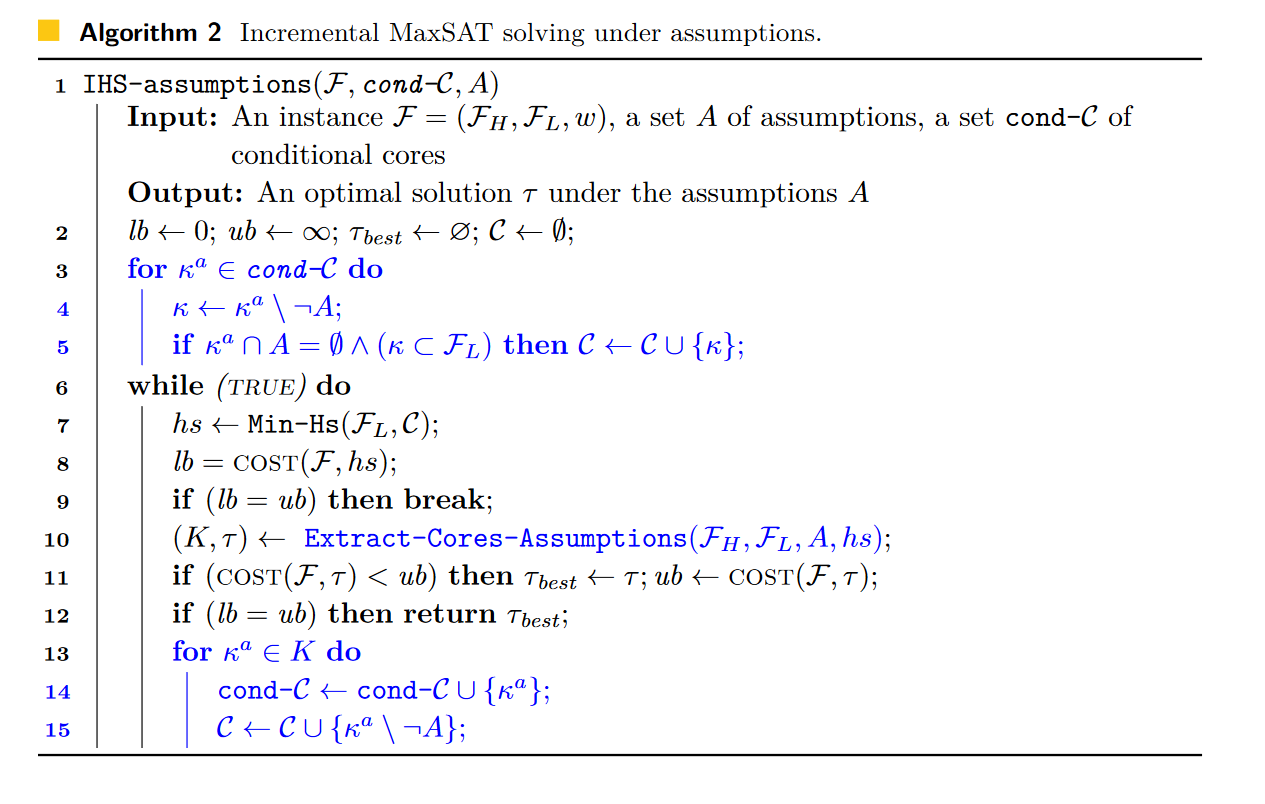
\includegraphics[width=0.73\linewidth]{8.png}
	\end{figure}
\end{frame}

\begin{frame}
	\frametitle{In theory}
With current MaxSAT assumptions $A$ :
	\begin{itemize}
		\item Include $A$ in the assumptions of every internal SAT solver call (and remove conflicting soft literals)
		\begin{itemize}
			\item models reported by the SAT solver will satisfy $A$
		\end{itemize} \pause
		\item SAT solver extracts conditional cores $\kappa^a$
		\begin{itemize}
			\item add $\kappa^a$ to a set of all collected conditional cores
			\item add the restriction $\kappa^a \backslash \neg A$ to the IP solver
		\end{itemize} \pause
	\end{itemize} \pause
	With next MaxSAT assumptions $A^{\prime}$ :
	\begin{itemize}
		\item Reinitialize the IP solver
		\item Check all known conditional cores $\kappa^a$
		\begin{itemize}
			\item if $\kappa^a \cap A^{\prime}=\emptyset$ and the restriction $\kappa^a \backslash \neg A^{\prime} \subseteq S$, add the restriction to the IP solver
		\end{itemize}
	\end{itemize} \pause
	No need to reinitialize the SAT solver, and cores are preserved.
\end{frame}

\begin{frame}
	\frametitle{Example 1}
	\begin{figure}[htbp]
		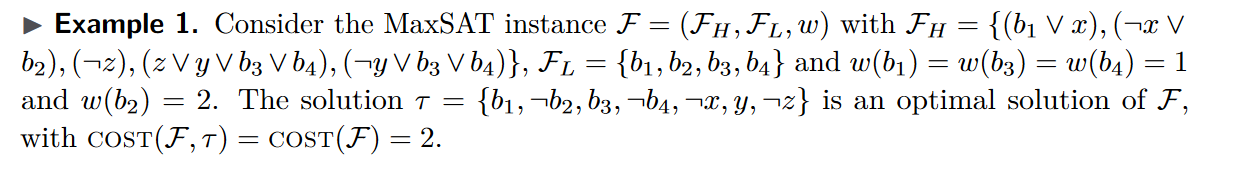
\includegraphics[width=1\linewidth]{1.png}
	\end{figure}
\end{frame}

\begin{frame}
	\frametitle{Example 4}
	\begin{figure}[htbp]
		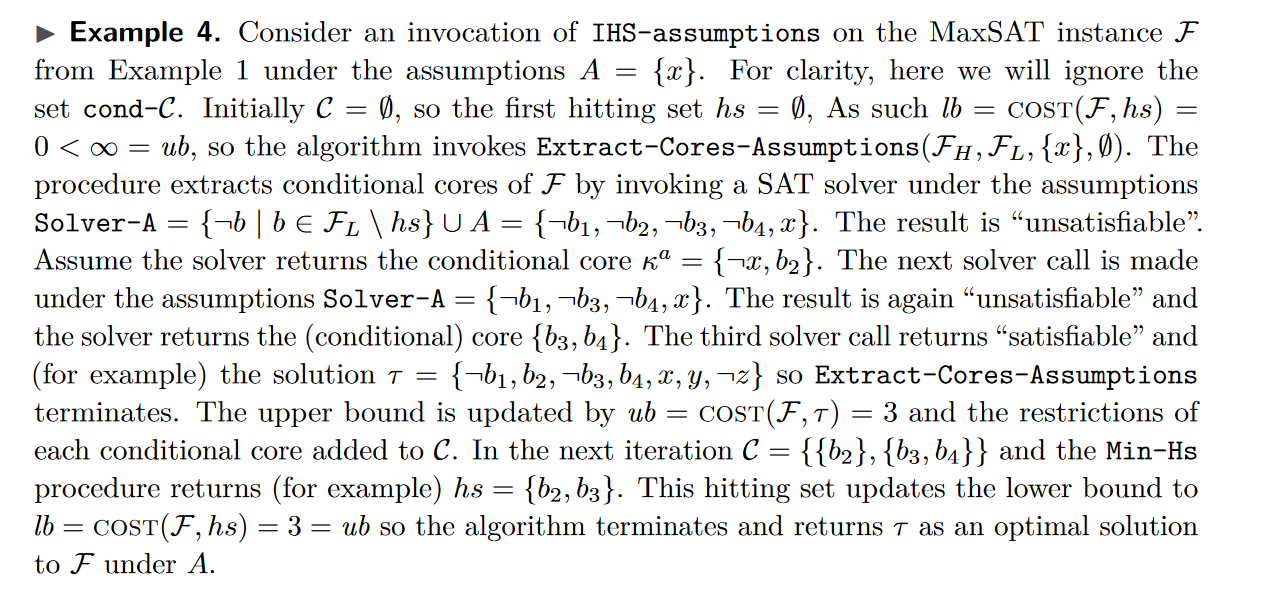
\includegraphics[width=.8\linewidth]{9.png}
	\end{figure}
\end{frame}

\begin{frame}
	\frametitle{In practice}
	Make use of \textbf{MaxHS: state-of-the-art IHS-based MaxSAT solver}. Realizing incrementality requires a non-trivial amount of engineering.
	\begin{itemize}
		\item \textbf{Maintaining conditional cores:} use another SAT solver as a database for storing conditional cores. To extract valid cores, perform unit propagation under current MaxSAT assumptions.
		\begin{itemize}
			\item removes redundant cores and simplifies them
			\item still need to check that the resulting cores only contain soft literals
		\end{itemize} \pause
		\item \textbf{IPAMIR wrapper:} When initialized, MaxHS performs several rounds of simplification to the input formula.
		\begin{itemize}
			\item variable mappings must be maintained
			% \item fixed literals need to be handled correctly
			% \item no pure literal elimination can be performed
		\end{itemize} 
	\end{itemize}
\end{frame}

\section{Empirical Evaluation}
\begin{frame}
	\frametitle{Empirical Evaluation}
	\begin{itemize}
		\item Benchmark instances
		\begin{itemize}
			\item All 1184 instances from complete tracks of MaxSAT Evaluation 2021
			\item For each benchmark, create 20 different sets of assumptions by hardening each soft clause with probability $0.01$.(23680 iterations overall)
		\end{itemize} \pause
		\item Benchmark setup
		\begin{itemize}
			\item iMaxHS vs. its non-incremental version in default settings
			\begin{itemize}
				\item for non-incremental, add assumptions directly as hard clauses
			\end{itemize}
			\item Per-instance limits: 7200 seconds and 16 GB memory
			\begin{itemize}
				\item instance: 20 MaxSAT solver calls each with different assumptions
				\item exclude WCNF parsing times from consideration
			\end{itemize}
			% \item no pure literal elimination can be performed
		\end{itemize} 
	\end{itemize}
\end{frame}

\begin{frame}
	\frametitle{Result}
	\begin{figure}[htbp]
		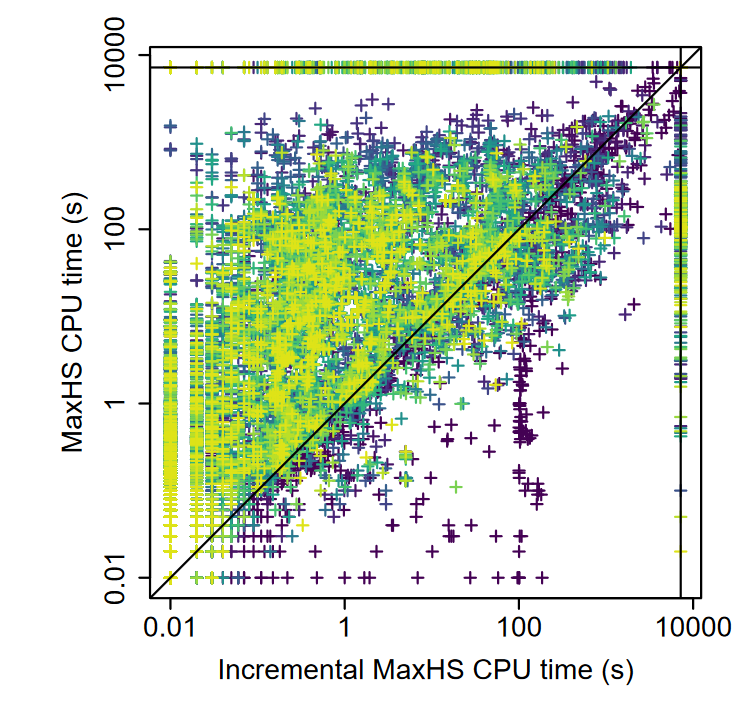
\includegraphics[width=.42\linewidth]{10.png}
	\end{figure}
\end{frame}

%------------------------------------------------


%------------------------------------------------

%------------------------------------------------


%------------------------------------------------
\begin{frame}
\hfill
\center{\Huge{\calligra{\Huge{Thank you}}}}
\linespread{3}\selectfont
\end{frame}
%----------------------------------------------------------------------------------------
\end{document}